\documentclass{standalone}
\usepackage{tikz}
\usepackage{ctex,siunitx}
\setCJKmainfont{Noto Serif CJK SC}
\usepackage{tkz-euclide}
\usepackage{amsmath}
\usepackage{wasysym}
\usetikzlibrary{patterns, calc}
\usetikzlibrary {decorations.pathmorphing, decorations.pathreplacing, decorations.shapes,}
\begin{document}
\small
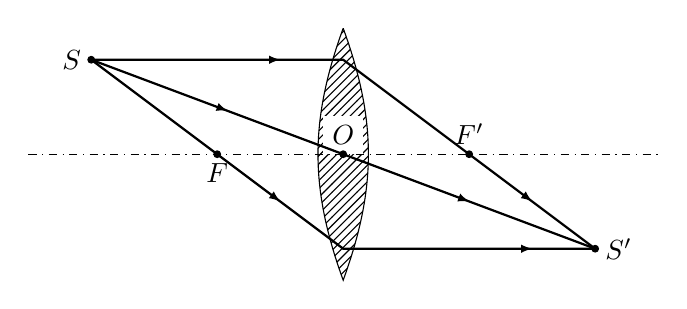
\begin{tikzpicture}[>=latex,scale=0.8]
  \draw [pattern=north east lines] (0,2) to [bend left=20] (0,-2) to [bend left=20](0,2);
  \node at (0,0)[fill=white, above]{$O$};
  \draw [dashdotted] (-5,0)--(5,0);
  \draw[thick] (-4,1.5)node[left]{$S$}--(0,1.5)--(2,0)--(4,-1.5)node[right]{$S'$};
  \draw[thick] (-4,1.5) --(0,-1.5)--(4,-1.5);
  \draw[thick] (-4,1.5)--(4,-1.5);
  \node at (2,0)[above]{$F'$};
  \node at (-2,0)[below]{$F$};
  \draw (-4,1.5) [fill=black] circle (1.5pt);
  \draw (4,-1.5) [fill=black] circle (1.5pt);
  \draw (0,0) [fill=black] circle (1.5pt);
  \draw (-2,0) [fill=black] circle (1.5pt);
  \draw (2,0) [fill=black] circle (1.5pt);
  \draw [->](-3,1.5)--(-1,1.5);
  \draw [->](1,-1.5)--(3,-1.5);
  \draw [->](-2,0)--(-1,-1.5/2);
  \draw [->](2,0)--(3,-1.5/2);
  \draw [->](0,0)--(2,-1.5/2);
  \draw [>-](-2,1.5/2)--(0,0); 
\end{tikzpicture}
\end{document}